\documentclass[runningheads]{llncs}

\usepackage[T1]{fontenc}
\usepackage{graphicx}
\usepackage{url}
\usepackage{booktabs}
\usepackage[inline]{enumitem}
\usepackage{listings}
%\usepackage[subtle]{savetrees}
\usepackage{xcolor}
\usepackage{microtype}
\usepackage{hyphenat}
\ttfamily\hyphenchar\font=45\relax\normalfont

% per overview
\usepackage{tikz}
\usetikzlibrary{arrows.meta,positioning}

% Code listing style for shell commands and file paths
\lstdefinestyle{shell}{
  basicstyle=\ttfamily\small,
  breaklines=true,
  frame=single,
  backgroundcolor=\color{gray!8},
  xleftmargin=3pt,
  xrightmargin=3pt,
  aboveskip=6pt,
  belowskip=4pt,
}

\renewcommand{\c}[1]{\textbf{\textcolor{red}{#1}}}

\begin{document}
\emergencystretch=2em
\tolerance=1000

\title{Artifact for `Assessing the Robustness of LLM-Based Oracles for Blockchain-Based Services'}
\titlerunning{Artifact: Robustness of LLM-Based Blockchain Oracles}

\author{Anonymous Authors}

\maketitle

\begin{abstract}
This paper presents the artifact accompanying the study \emph{``Assessing the Robustness of LLM-Based Oracles for Blockchain-Based Services''}, accepted at ICSOC~2026. The artifact contains the complete experimental pipeline, benchmark question datasets, pre-computed simulation traces across 64~configurations (covering four LLM families, four decoding temperatures, two node splits, and two datasets), baseline implementations (Astraea and DeepThought), and statistical analysis scripts for Honest Selection Rate, Final Credibility Delta, and Sustained Credibility Dominance. An interactive Terminal User Interface (TUI) launcher is provided to facilitate artifact evaluation, supporting local verification of existing results without API credentials as well as full end-to-end replication.
\end{abstract}

\keywords{Blockchain Oracles \and Large Language Models \and Collusion Attacks \and Reputation Systems \and Replication Package.}

\section{Introduction}
\label{sec:introduction}
This artifact accompanies the paper \emph{`Assessing the Robustness of LLM-Based Oracles for Blockchain-Based Services'}, accepted as a full paper at ICSOC~2026. The study evaluates C-LLM~\cite{xian2024cllm}, a representative LLM-based blockchain oracle, under coordinated minority attacks in which malicious nodes submit semantically consistent but factually incorrect responses. The evaluation spans four LLM variants, four decoding configurations, two honest-to-malicious node splits, and two benchmark datasets, and includes a comparison with the human-based oracle baselines Astraea~\cite{adler2018astraea} and DeepThought~\cite{di2022deepthought}.

Figure~\ref{fig:artifact-overview} summarizes the artifact contents. The artifact is publicly available at:
\begin{center}
\url{https://doi.org/10.5281/zenodo.21430174}.
\end{center}


\begin{table}[t]
\centering
\caption{Artifact contents overview.}
\label{tab:contents}
\footnotesize
\begin{tabular}{lll}
\toprule
\textbf{Component} & \textbf{Type} & \textbf{Description} \\
\midrule
Experimental pipeline  & Code & 5-step Python pipeline for C-LLM evaluation \\
Astraea comparison     & Code & Analytical $q^*$ solver (binomial CDF) \\
DeepThought comparison & Code & Simulation engine (Python reimplementation) \\
MIX dataset            & Data & 100 open-ended questions, 10 domains \\
PRO dataset            & Data & 60 multiple-choice physics questions \\
Raw LLM responses      & Data & Answers from 4 LLM families $\times$ 4 configs $\times$ 2 splits \\
Credibility logs       & Data & Node weight evolution for every run and shuffle \\
Analysis results       & Data & Excel workbooks with aggregate metrics \\
README                 & Docs & Step-by-step reproduction guide \\
\bottomrule
\end{tabular}
\end{table}

\begin{figure}[t]
\centering
\resizebox{\textwidth}{!}{%
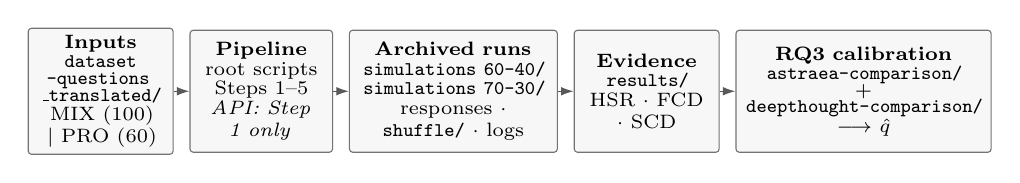
\begin{tikzpicture}[
  stage/.style={
    draw=black!55,
    fill=black!3,
    rounded corners=1.2pt,
    align=center,
    minimum height=1.55cm,
    inner xsep=2pt,
    inner ysep=2.5pt,
    font=\scriptsize
  },
  flow/.style={
    -{Latex[length=1.6mm,width=1.1mm]},
    draw=black!65,
    line width=0.45pt
  },
  node distance=2mm
]

% Input datasets
\node[stage, text width=1.7cm] (inputs) {
  \textbf{Inputs}\\[-1pt]
  {\ttfamily dataset}\\[-2pt]
  {\ttfamily -questions}\\[-2pt]
  {\ttfamily \_translated/}\\[-1pt]
  MIX (100) $\mid$ PRO (60)
};

% Five-step pipeline
\node[stage, text width=1.67cm, right=of inputs] (pipeline) {
  \textbf{Pipeline}\\[-1pt]
  root scripts\\[-1pt]
  Steps 1--5\\[-1pt]
  \emph{API: Step 1 only}
};

% Archived configuration outputs
\node[stage, text width=2.5cm, right=of pipeline] (runs) {
  \textbf{Archived runs}\\[-1pt]
  {\ttfamily simulations 60-40/}\\[-1pt]
  {\ttfamily simulations 70-30/}\\[-1pt]
  responses $\cdot$ \texttt{shuffle/} $\cdot$ logs
};

% RQ1--RQ2 evidence
\node[stage, text width=1.7cm, right=of runs] (results) {
  \textbf{Evidence}\\[-1pt]
  {\ttfamily results/}\\[-1pt]
  HSR $\cdot$ FCD $\cdot$ SCD
};

% RQ3 branch
\node[stage, text width=3.1cm, right=of results] (rqthree) {
  \textbf{RQ3 calibration}\\[-1pt]
  {\ttfamily astraea-comparison/}\\[-2pt]
  $+$\\[-2pt]
  {\ttfamily deepthought-comparison/}\\[-1pt]
  $\longrightarrow$ $\hat q$
};

\draw[flow] (inputs) -- (pipeline);
\draw[flow] (pipeline) -- (runs);
\draw[flow] (runs) -- (results);
\draw[flow] (results) -- (rqthree);

\end{tikzpicture}%
}
\caption{Artifact organization and verification flow
(only Step~1 requires LLM APIs).}
\label{fig:artifact-overview}
\end{figure}


\section{Repository Structure and Getting Started}
\label{sec:structure}
The repository is organized as follows. The root directory contains the interactive replication launcher (\texttt{tui\_launcher.py} and accompanying \texttt{tui/} package), the five Python scripts that implement the experimental pipeline (Section~\ref{sec:pipeline}), plus dependency and license files. The \texttt{dataset-questions\_translated/} directory holds the two benchmark datasets in JSON format: \texttt{q\_100\_MIX.json} (100~open-ended questions across ten domains) and \texttt{q\_60\_PRO.json} (60~multiple-choice physics questions at three educational levels). Both were translated from the original Chinese datasets used in the C-LLM evaluation~\cite{xian2024cllm}; originals are in \texttt{utility/BASE/}.

Pre-computed results are organized under \texttt{simulations~60-40/} and \texttt{simulations~70-30/}, one directory per node split. Each subdirectory follows the naming convention \texttt{$\langle$decoding$\rangle$\_run\_$\langle$dataset$\rangle$\_$\langle$model$\rangle$/} and contains: the question file (\texttt{q\_*.json}), the collected LLM responses (\texttt{q\_*\_answers.json}), the single-run credibility log (\texttt{node\_weights\_log\_run\_*.txt}) and a \texttt{shuffle/} subdirectory with 20 or 30 shuffled answer files and corresponding credibility logs. The \texttt{results/} directory contains the aggregated Excel workbooks and the analysis scripts for Final Credibility Delta (\texttt{compute\_fcd\_ci.py}) and Sustained Credibility Dominance (\texttt{compute\_scd.py}). Baseline comparison code resides in \texttt{astraea-comparison/} and \texttt{deepthought-comparison/}.

\subsection{Installation}
\label{sec:installation}

The artifact requires Python~3.9 or later. Installation proceeds via a standard virtual environment:

\begin{lstlisting}[style=shell]
python3 -m venv .venv && source .venv/bin/activate
pip install -r requirements.txt
\end{lstlisting}

\noindent LLM API keys (OpenAI, Google GenAI, DeepSeek) are required \emph{only} for Step~1 of the pipeline. All subsequent steps, analysis scripts and baseline comparisons run entirely locally.


\section{Step-by-Step Reproduction Guide}
\label{sec:pipeline}
\subsection{Interactive Replication Launcher (TUI)}
\label{sec:tui}

To eliminate manual script configuration and streamline verification for artifact reviewers, the repository includes an interactive Terminal User Interface (TUI) launcher:

\begin{lstlisting}[style=shell]
python3 tui_launcher.py
\end{lstlisting}

\noindent The launcher provides two operational workflows:
\begin{itemize}
    \item \textbf{Verify Existing Results (Recommended for Artifact Evaluation):} The user selects any of the evaluated models, datasets, splits, and decoding configurations. The tool copies the corresponding pre-computed raw answer file into an isolated workspace (\path{replication/}, git-ignored) and runs Steps~2--5 locally. This validates the pipeline without requiring API keys or external network requests.
    \item \textbf{Full Replication:} The user interactively selects the model, dataset, split, and decoding configuration, inputs their API key, and executes Steps~1--5 end-to-end.
\end{itemize}

\subsection{Manual Step-by-Step Execution}
\label{sec:manual-pipeline}

Alternatively, reviewers can execute each step manually via the CLI as described below. Pre-computed outputs for all 64 configurations are included in the repository, so reviewers may skip Step~1 and start from any subsequent step.

\smallskip\noindent\textbf{Step 1: LLM Response Generation (requires API keys).} The script \texttt{generate\_answers.py} queries the designated LLM, which can be configured along with its API key, to generate honest responses from $N$~honest nodes and two additional example responses. It then constructs a malicious prompt (Figure~2 in the original paper) that instructs the LLM to produce a factually incorrect but stylistically matched answer, which is replicated across all malicious nodes to simulate perfect collusion. The user configures the LLM provider and API key (lines~6--27), experiment parameters (lines~30--47) and runs:

\begin{lstlisting}[style=shell]
python3 generate_answers.py
\end{lstlisting}

\noindent\textbf{Output}: \texttt{q\_*\_answers.json}, a JSON array where each entry contains a question and 10 answers (first $N$ honest, last $10{-}N$ colluded malicious). The script supports crash-safe incremental saving and automatic resume from partial runs.

\smallskip\noindent\textbf{Step 2: Question Order Shuffling.} The script \texttt{shuffle.py} generates randomized permutations of the question order (30 for MIX, 20 for PRO) to account for sequential credibility-update effects. Configuration is set in lines~11--14.

\begin{lstlisting}[style=shell]
python3 shuffle.py
\end{lstlisting}

\smallskip\noindent\textbf{Step 3: Single-Run Credibility Computation.} The script \texttt{calc\_cred.py} implements the C-LLM aggregation mechanism. For each question, it encodes the 10~node responses into \texttt{bert\mbox{-}base\mbox{-}uncased} embeddings (mean pooling over the last hidden state), computes pairwise cosine similarity and updates node credibility weights following the C-LLM procedure. It also persists the computed similarity matrix (\texttt{similarity\_cache.pkl}) to accelerate multi-run permutations. Configuration is set in lines~73--75.

\begin{lstlisting}[style=shell]
python3 calc_cred.py
\end{lstlisting}

\noindent\textbf{Output}: \texttt{node\_weights\_log\_run\_*.txt}, one line per question, 10~space-separated weight values. Columns~1--$N$ correspond to honest nodes; columns~$N{+}1$--10 to malicious nodes. The script defaults to CPU for numerical reproducibility (${\sim}$15--30\,s on modern CPUs).

\smallskip\noindent\textbf{Step 4: Multi-Run Credibility Computation.} The script \texttt{calc\_cred\_shuffle.py} executes credibility updates across all shuffled orderings. By leveraging the cached similarity matrix computed in Step~3, it bypasses redundant neural embeddings while strictly recomputing credibility dynamics for each permutation ($<$2\,s total).

\begin{lstlisting}[style=shell]
python3 calc_cred_shuffle.py
\end{lstlisting}

\smallskip\noindent\textbf{Step 5: Excel Report Generation.} The script \texttt{generate\_excel.py} compiles weight logs into Excel workbooks with single-run and shuffled-run sheets, computing the per-run Honest Selection Rate (HSR), credibility-delta sequences, and aggregate statistics (minimum, maximum, and mean). Output workbooks produced by the replication pipeline are saved as \texttt{$\langle$decoding$\rangle$\_Research-project\_$\langle$model$\rangle$\_replication.xlsx} in \path{replication/results/}, allowing concurrent side-by-side inspection with baseline workbooks.

\begin{lstlisting}[style=shell]
python3 generate_excel.py
\end{lstlisting}


\section{Analysis Scripts and Baseline Reproduction}
\label{sec:analysis}
Reviewers can evaluate the post-pipeline metrics and human-oracle baselines either interactively via the TUI launcher (selecting ``Run Analysis'' after pipeline execution) or by executing the standalone scripts via CLI. When using the TUI, the interface auto-populates available Excel workbooks from both \path{replication/results/} and repository \path{results/}.

\smallskip\noindent\textbf{Final Credibility Delta (FCD) with 95\% CI.} The script \texttt{results/compute\_fcd\_ci.py} extracts the final credibility delta from each shuffled run in an Excel workbook and computes the mean, sample standard deviation and 95\% confidence interval using Student's $t$-distribution. It requires an Excel workbook generated by Step~5 (or any pre-computed workbook in \texttt{results/}):

\begin{lstlisting}[style=shell]
python3 results/compute_fcd_ci.py results/<workbook>.xlsx
\end{lstlisting}

\smallskip\noindent\textbf{Sustained Credibility Dominance (SCD).} The script \texttt{results/compute\_scd.py} detects the first step at which the aggregate credibility of malicious nodes exceeds that of honest nodes for at least 10~consecutive steps, reporting incidence and mean onset. Like FCD, it takes a Step~5 Excel workbook as input:

\begin{lstlisting}[style=shell]
python3 results/compute_scd.py results/<workbook>.xlsx
\end{lstlisting}

\smallskip\noindent\textbf{Astraea Baseline (RQ3).} The script \texttt{astraea-comparison/q-star.py} computes the honest-reporter competence $\hat{q}$ ($q^*$ in code) required for Astraea's staking-based voting mechanism to match C-LLM's Honest Selection Rate, using the analytical binomial model from the original Astraea paper~\cite{adler2018astraea}. It requires no external arguments and reads directly from the pre-computed HSR values:

\begin{lstlisting}[style=shell]
python3 astraea-comparison/q-star.py
\end{lstlisting}

\smallskip\noindent\textbf{DeepThought Baseline (RQ3).} The \texttt{deepthought-comparison/} directory contains an adaptation of the original DeepThought implementation~\cite{di2022deepthought}, reproducing the core decision process while excluding deployment and on-chain components (consistent with Section~4.1 of the main paper). The simulation engine (\texttt{deepthought\_sim.py}) accepts command-line arguments for dataset (\texttt{MIX} or \texttt{PRO}), split (\texttt{60-40} or \texttt{70-30}), and assumed human-reporter accuracy (\texttt{--accuracy}, default: $0.8$):

\begin{lstlisting}[style=shell]
python3 deepthought-comparison/deepthought_sim.py \
    --dataset MIX --split 60-40 --accuracy 0.8
\end{lstlisting}

\noindent After executing the simulation, the aggregation and report script produces summary CSVs, an Excel comparison report, PNG charts, and empirical $\hat{q}$ values via curve interpolation:

\begin{lstlisting}[style=shell]
python3 deepthought-comparison/generate_results.py --results-dir results
\end{lstlisting}

\noindent All pre-computed DeepThought outputs are archived in \path{deepthought-comparison/results/} for immediate verification.


\section{Data Description and Provenance}
\label{sec:data}
\noindent\textbf{Datasets.} Both benchmark datasets originate from the C-LLM evaluation~\cite{xian2024cllm} and were automatically translated from Chinese to English. \emph{MIX} contains 100~open-ended questions spanning ten domains (science, history, mathematics, language, culture, geography, entertainment, technology and personal/conversational topics). \emph{PRO} contains 60~four-option multiple-choice physics questions stratified across three educational levels: Junior High School (20), High School (20) and University (20). Both are stored as JSON arrays with fields \texttt{question} and \texttt{answer}. Binary yes/no variants used by the DeepThought baseline are in \texttt{deepthought-comparison/datasets/}.

\smallskip\noindent\textbf{Experimental Configurations.} Table~\ref{tab:configs} summarizes the 64~configurations evaluated in the paper. Each configuration is uniquely identified by the combination of LLM model, decoding setting, dataset and node split. The evaluated LLMs are ChatGPT-4o-mini, Gemini-2.5-flash-lite (configured with 8192 output tokens and reasoning disabled) and DeepSeek-v4-flash in two inference modes: \emph{non-thinking} (referred to as chat) and \emph{thinking} (referred to as reasoner). The directory naming convention maps directly to these parameters.

\begin{table}[t]
\centering
\caption{Experimental configurations (64 total = 4 $\times$ 4 $\times$ 2 $\times$ 2).}
\label{tab:configs}
\footnotesize
\begin{tabular}{llcl}
\toprule
\textbf{Dimension} & \quad\textbf{Values} & \textbf{Count} \\
\midrule
LLM family & \quad GPT-4o-mini, Gemini-2.5-flash-lite, & 4 \\
           & \quad DeepSeek-v4-flash (chat, reasoner) & \\
Decoding   & \quad $C_1$: $T{=}0$; $C_2$: $T{=}0.5$; & 4 \\
           & \quad $C_3$: $T{=}1.0$; $C_4$: $T{=}1.0$, seed$=4321$ & \\
Dataset    & \quad MIX (100\,Qs, 30 runs), PRO (60\,Qs, 20 runs) & 2 \\
Node split & \quad 6/4 (60-40), 7/3 (70-30), $N{=}10$ & 2 \\
\bottomrule
\end{tabular}
\end{table}


\smallskip\noindent\textbf{LLM Responses.} For each configuration, the repository includes the complete set of LLM-generated answers in JSON format. Each entry in \texttt{q\_*\_answers.json} contains a question string and an array of 10~answers: the first $N$~are independently generated honest responses, the remaining $10{-}N$ are identical copies of the coordinated malicious response produced via the adversarial prompt (Figure~2 in the original paper).

\smallskip\noindent\textbf{Credibility Logs.} The files \texttt{node\_weights\_log\_*.txt} record the evolution of node credibility across questions. Each line contains 10~floating-point values representing the updated credibility of each node after processing one question. The credibility update follows the C-LLM procedure: BERT embeddings (\texttt{bert-base-uncased}, mean pooling) are used to compute pairwise cosine similarity, which is then combined with current node weights to produce updated weights. All nodes are initialized at $0.50$, as per the original C-LLM evaluation~\cite{xian2024cllm} .

\smallskip\noindent\textbf{Analysis Reports.} The \texttt{results/} directory contains 16~Excel workbooks (one per model $\times$ decoding configuration) plus a cross-model dashboard. Each workbook includes sheets for single-run weight evolution, shuffled-run weight evolution, per-run accuracy and credibility delta sequences. Statistical summaries (FCD with 95\% CI, SCD incidence) are in the \texttt{final-deltas/} and \texttt{systemic-dominance/} subdirectories.

\smallskip\noindent\textbf{SBERT Model.} The credibility computation uses \texttt{bert-base-uncased}, consistent with the Sentence-BERT approach described in Reimers and Gurevych~\cite{reimers2019sbert}. Sentence embeddings are obtained via mean pooling over the last hidden state. The model is automatically downloaded (${\sim}$440\,MB) on first execution of Step~3.


\section{Requirements, Limitations, and License}
\label{sec:limitations}
\smallskip\noindent\textbf{Cloud Service Requirements.} Step~1 requires API access to the LLM providers (OpenAI, Google GenAI, DeepSeek). Each provider requires a registered account and a valid API key, which must be configured in \texttt{generate\_answers.py} (or supplied interactively via the TUI launcher) before execution. The pre-computed LLM responses included in the repository enable complete verification of Steps~2--5 and all metrics without API access.

\noindent\textbf{Software and Hardware Requirements.} The artifact requires Python~3.9+ and the packages listed in \texttt{requirements.txt}. Steps~2--5 and all analysis scripts run on any standard hardware. Step~3 downloads the \texttt{bert-base-uncased} model (${\sim}$440~MB) on first execution and uses CPU by default for deterministic results; optional GPU acceleration is supported via environment variables (\texttt{BERT\_DEVICE=mps} for Apple Silicon, \texttt{BERT\_DEVICE=cuda} for NVIDIA GPUs).

\smallskip\noindent\textbf{Non-Determinism.} LLM APIs are inherently non-deterministic: repeated calls with identical parameters may yield different textual outputs. As discussed in Section~6 (Threats to Validity) of the main paper, the numerical values of individual metrics may vary across executions, but the qualitative findings and trends reported in the paper remain stable across the multiple runs performed.

\smallskip\noindent\textbf{Verification Without API Keys.} Reviewers who do not have API keys can verify the artifact as follows: (i)~install the dependencies and run the analysis scripts (\texttt{compute\_fcd\_ci.py}, \texttt{compute\_scd.py}) on the included Excel workbooks to confirm the reported metrics; (ii)~re-run Steps~3--5 on the pre-computed answer files to verify that the credibility computation and report generation produce consistent results; (iii)~run the Astraea and DeepThought baselines locally (no API keys required) to verify the RQ3 comparison.

\smallskip\noindent\textbf{License.} The artifact code, reproduction scripts, benchmark datasets, and analysis routines are distributed under the open-source MIT License (see \texttt{LICENSE} in the repository root).



\bibliographystyle{splncs04}
\bibliography{references}

\end{document}
